This chapter describes the methods used when implementing the algorithms used to solve the problem, and the evaluation of the outcome.

\section{Implementation}
This section presents the methods use when implementing the algorithms used to solve the problem. % Todo rephrase

\subsection{Software used}
The most important piece of software used is the library OpenCV. % footnote to opencv homepage?
OpenCV is an open source library for computer vision, which is used extensively in this thesis. 
It contains functions for many things that one needs when working with computer vision-related fields, from low-level processing such as filters, to high-level functions for feature detection and machine learning.
OpenCV is written in C/C++, but also has full interfaces for python, java and MATLAB\cite{wiki:OpenCV}.
\subsection{Hardware used}
The hardware used to capture test pictures and run the test app is a Samsung Galaxy S6 Edge, which is an Android smartphone.
The S6 Edge was chosen because it currently tops benchmarks and tests, both regarding processing power and photo quality \cite{phone_performance_benchmark}\cite{phone_camera_benchmark}.

\subsection{Android Application}
A simple proof of concept android application was made for online testing on the phone, to test the speed of the measuring algorithm.
The app simply displays the camera feed and continuously feeds new frames to the measuring algorithm.
When the package or reference object is successfully detected, an overlay is drawn to outline their position on the screen.
If both the package and reference are found in the same frame, the dimensions of the package are calculated, and each dimension is drawn next to the appropriate edge.
The processing time for each frame is also displayed.
% TODO Add figure!

\subsection{Preprocessing}

Preprocessing is the first step in most computer vision algorithms. 
Its purpose here is to reduce noise. 
This is accomplished by converting the colour image to a grayscale image, followed by applying a median filter. 
A median filter was chosen because it reduces noise effectively, while also removing small, unwanted features from the image, such as small labels and marks on the package or the rest of the scene. 
At the same time well defined edges are preserved.

\subsection{Line detection} % TODO write
The next step is to detect edges in the image. This is done using Canny's edge detection algorithm. As it is often a good pr
To reduce amount of data contours are pruned by removing peripheral contours and short ones.
Lines are detected by using the Hough Line Transform.

\subsection{Package Detection}

The algorithm used to detect the package is based on a ranking scheme, where multiple hypothesis about where the package is are created, and then scored. 
The candidate with the highest score is chosen as the package. 

A fundamental property of cuboids is exploited by the algorithm: they consist of parallel line segments of equal length. 
More specifically, the outline of a cuboid in a two dimensional image is made up of three pairs of parallel line segments, which form a hexagon. 
However because of perspective distortion the line segments will not be entirely parallel, and not  of exactly equal length.
This is where the ranking algorithm comes in.
The assumption that the package is the most symmetric hexagon in the image is made. % TODO not quite true, reformulate
Thus, the ranking algorithm rates a package candidate according to the degree of parallelism and equality of lengths between opposing sides.

The first step is, however, to find the candidates.
This is done by first finding pairs of parallel line segments. 
As mentioned above, the line segments will not be exactly parallel, due to perspective distortion. % TODO perspective distortion correct term? 
Thus a pair of line segments is considered to be parallel by the algorithm if the angle between them is below a threshold. 
This threshold is set to be high, to avoid discarding a pair that belongs to the actual package, since the perspective distortion is rather large from some perspectives. % TODO be more specific? example? max distortion?

The next step is to pick three pairs of parallel line segments and let their intersections form a polygon. 
Since the full contour of the package is not always distinguishable, the sought intersections are those between the lines (i. e. does not have a start or end point) defined by the line segments, not the line segments themselves. % elaborate, distinguishable from what? only some intersections are considered
The polygon is considered to be a candidate if it passes some basic tests, for example it must be convex and have six corners. 
The corner must also be within the bounds of the image.
Additionally, if the location of the reference object is known, the package must enclose the reference object.
This is done for all combinations of three parallel line pairs.
% Additional constraints... 

When all candidates are generated they are scored according to the rules rules presented above.

\subsection{Reference Object Detection}

The reference object is detected using a modified version of the package detection algorithm.
Since the reference object is a quadrilateral two pairs of parallel line segments are picked out at a time to form a quadrilateral.
The ranking algorithm also uses some additional criteria, since the reference object is a white ISO 216 A-series  paper, the score is also based on how bright the area within the polygon is, and how well the aspect ratio between the two sides matches that of a ISO 216 A-series paper.

\subsection{Measuring}

The measuring is carried out in two steps, first the width and depth of the package are measured, followed by the height. 
This reason behind this order is that the reference object is placed on top of the package, which means that there is some special information about the top plane, and top corners, of the package.

As described in \ref{planar-homographies} the world coordinate system can be defined to have its origin in one of the corners of the reference object.
Since the physical size of the reference object is known, the position of all corners is known in both image, and world coordinates.
With the four point correspondences, a planar homography is estimated, which can be used to map any point in the image its corresponding point in the plane.
The position of the four top corners of the package can now be calculated, along with the width and depth, by calculating the euclidean distance between the world coordinates of the corners.

Now, all that is needed is the position of one (or more) of the lower corners of the package, in world coordinates.
A homography cannot be created in the same way between the image plane and the side planes of the package, since the world coordinates of only two points is known in either of the side planes.
This is why camera calibration is useful, because with it, points can be projected with equation \ref{eq:projection1}.

As discussed in \ref{problem-statement} two types of calibrations are to be implemented, one using an offline configuration which must be done beforehand, and one using online calibration.
The offline configuration is implemented using Zhang's method.
A checkerboard pattern of squares with known size is printed out on a regular A4 paper.
Then, multiple images are taken of the pattern, from different perspectives. 
The images are then fed to the algorithm which outputs an estimate of $K$.% TODO refer to opencv implementation in footnote?

\begin{figure}[h]
\begin{center}
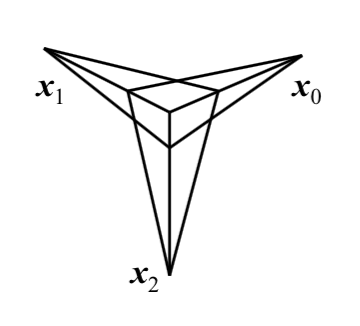
\includegraphics[width=0.4\textwidth]{figures/vanishing_points.png}
\end{center} % TODO bättre fig text?
\caption{Visualisation of how the edges of a cuboid give rise to three orthogonal vanishing points.} % TODO hur referera? Tagen från szeliski s. 330
\label{fig:vanishing_points}
\end{figure}

The online configuration uses vanishing point calibration.
It is ideal to use vanishing point calibration for this particular problem since every cuboid package has three orthogonal sets of parallel lines which result in three orthogonal vanishing points.
Additionally, the known homography between the image plane and the top-plane of the package can be used to improve the estimate of $K$.

When the $K$ is known, the camera pose can be estimated as described in \ref{camera-pose}, using the four image-world point correspondences given by the reference object.
The EPnP is chosen, because it appears to be the current state-of-the-art. % TODO refer opencv?

Once the camera pose is obtained, equation \ref{eq:projection1} can be used, which means that any point in the world can be projected to a point in the image.
However, the reverse mapping is sought, i.e. the position of the package the world of the image coordinates of the bottom corners of the package, i.e. the reverse mapping.
This is generally not possible to do, unless something is known about the geometry of the scene.
Luckily, it is known that the lower corners share $X$, and $Y$ coordinates with a top corner, which position is already known.
The image coordinates $(u,v)$ of a lower corner, and the world coordinates $(X,Y)$ of the corresponding upper corner can then be used to solve for the $Z$ coordinate of the lower corner. 
Equation \ref{eq:projection3} can be transformed to the following over-defined system:
\begin{equation} \label{eq:constrained-projection}
\begin{pmatrix} up_{33}-p_{13} \\ vp_{33}-p_{23} \end{pmatrix} Z = 
\begin{pmatrix}
X(p_{11}-up_{31}) + Y(p_{12}-up_{32})+p_{14}-u \\
X(p_{21}-vp_{31}) + Y(p_{22}-vp_{32})+p_{24}-v
\end{pmatrix}
\end{equation}
This is solved as a least-squares problem using Single Value Decomposition (SVD).
Since two pairs of upper-lower corners which share $X$ and $Y$ coordinates are known, two least-squares solutions of $Z$ can be obtained.
The solution with the smallest error is chosen as $Z$.



